%
% LaTeX report template 
%
\documentclass[a4paper,10pt]{article}
\usepackage{graphicx}
\usepackage[english]{babel}
\usepackage[latin1]{inputenc}
\usepackage{cite}
\usepackage[table]{xcolor}
%
\begin{document}
%
   \title{Matrices with Matlab}

   \author{Isaiah Martinez \\ CSUN \\ Mathematics Department \\ isaiah.martinez.891@my.csun.edu}
          
   \date{02/3/2021}

   \maketitle
   
   \tableofcontents
 
  \newpage
    
% This is a comment: in LaTeX everything that in a line comes
% after a "%" symbol is treated as comment
%\section*{Foreword}
% When adding * to \section, \subsection, etc... LaTeX will not assign
% a number to the section
%When writing a scientific report it is very important to think
%carefully how to organize it.
%Most reports and scientific papers follow the so called IMRAD structure,
%that is they are subdivided in four sections: \textbf{I}ntroduction, 
%\textbf{M}ethods, \textbf{R}esults \textbf{A}nd \textbf{D}iscussion.
%This is a well-tried format and an efficient way of writing a report,
%it is highly recommended that you stick to it: 
%the goal of a report or a scientific paper is not to impress 
%the readers by poetic language but to transfer facts and new insights 
%as clearly as possible. 
%More importantly structuring your paper   
%helps you understand more about the topic you are examining.

%\paragraph{Note:}
%This document is not meant to be a tutorial for how to write
%a good scientific report, although it contains some useful advices.
%A more complete tutorial can be found on the web at the URL:
%\begin{verbatim}

%http://www.wisc.edu/writing/Handbook/ScienceReport.html

%\end{verbatim}
%You are highly encouraged to take a look at this web-site!

\section{Introduction}
[Background on the topic]

\begin{enumerate}
\item In the first section we will describe the process toward which the results of the project were obtained.
\item The section presents the results we obtained with...
\end{enumerate}

The introduction should state clearly why the study was started
and give a relatively short and essential overview of the topic
you are exploring. References to previous works can be made here.
 
The introduction should not contain the conclusions. 
At the end of the introduction the outline of the paper may be described.
 
 
\section{Methods}
Here you describe the strategy you adopted and the tools you
used in your study.
\subsection{Example of subsection}
This is a subsection.
\subsubsection{Example of subsubsection}
This is a sub-subsection.

\subsection{Example of mathematical formulas}
\LaTeX is a very powerful tool when it comes to typesetting of
mathematical equations. The quality of the output is extremely
high and hardly matched by other word processors. It takes little
time with {\LaTeX\,}  to learn how to handle 
even complicated mathematical expressions.
   \begin{eqnarray}
    %  \sigma_0 & = & \frac{\pi}{\sqrt{8}}
       %              \frac{1}{ \tau_{\mathrm{ff}}} \\
       f(x)& = & \frac{x + 1}{2x-3}\\
      K        & = & \frac{\sqrt{32}}{\pi} \frac{1}{\delta}
                        \frac{ \tau_{\mathrm{ff}} }
                             { \tau_{\mathrm{co}} } \nonumber \,;
   \end{eqnarray}

\begin{eqnarray} \label{eqn:demo5}
{\mathrm a} x^2 + {\mathrm b} x + {\mathrm c} = 0 \nonumber \\
{\mathrm d} x^2 + {\mathrm e} x + {\mathrm f} = 0 \nonumber 
\end{eqnarray}


\LaTeX\, uses a simple and convenient system for assigning numbered labels
to equations and other objects (figures, tables, etc\ldots) and for referring
to them. After having edited the source file and rearranged the position of
the equations, \LaTeX\, will  change labels and references
consistently throughout the text (if you did the things right of
course\ldots) 
 
Examples of text containing mathematical expressions and equations: 
   \[
      \begin{array}{lp{0.8\linewidth}}
         M_{r}  & mass internal to the radius $r$     \\
         m               & mass of the zone                    \\
         r_0             & unperturbed zone radius             \\
         \rho_0          & unperturbed density in the zone     \\
         T_0             & unperturbed temperature in the zone \\
         L_{r0}          & unperturbed luminosity              \\
         E_{\mathrm{th}} & thermal energy of the zone
      \end{array}
   \]

\noindent
    
   \begin{equation}
      \tau_{\mathrm{co}} = \frac{E_{\mathrm{th}}}{L_{r0}} \,,
   \end{equation}


   \begin{equation}
      \tau_{\mathrm{ff}} =
         \sqrt{ 
	 	\frac{3 \pi}{32 G} \frac{4\pi r_0^3}{3 M_{\mathrm{r}}}
	 }\,,
   \end{equation}


\begin{equation}
 \displaystyle \frac{dy}{dx} = \langle x^2 - y^2 \rangle
\end{equation}

\begin{equation}
  \frac{dy}{dx} = \left ( x^2 - y^2 \right )
\end{equation}

\begin{equation}
 \displaystyle \frac{dy}{dx} = [ x^2 - y^2 ]
\end{equation}

\begin{equation}
 \displaystyle \frac{\mathcal R dy}{\mathbf E dx} = \langle x^2 - y^2 \rangle
\end{equation}

   \begin{displaymath}
      \nabla_{\mathrm{ad}} = \left( \frac{ \partial \ln T}
                             { \partial\ln P} \right)_{S} \, , \;
      \chi^{}_T       = \left( \frac{ \partial \ln P}
                             { \partial\ln T} \right)_{\rho} \, , \;
      \kappa^{}_{T}   = \left( \frac{ \partial \ln \kappa}
                             { \partial\ln T} \right)_{T}
   \end{displaymath} 
   \begin{eqnarray}
      \frac{\pi^2}{8} \frac{1}{\tau_{\mathrm{ff}}^2}
                ( 3 \Gamma_1 - 4 )
         & > & 0 \label{ZSDynSta} \\
      \frac{\pi^2}{\tau_{\mathrm{co}}
                   \tau_{\mathrm{ff}}^2}
                   \Gamma_1 \nabla_{\mathrm{ad}}
                   \left[ \frac{ 1- 3/4 \chi^{}_\rho }{ \chi^{}_T }
                          ( \kappa^{}_T - 4 )
                        + \kappa^{}_P + 1
                   \right]
        & > & 0 \label{ZSSecSta} \\
     \frac{\pi^2}{4} \frac{3}{\tau_{ \mathrm{co} }
                              \tau_{ \mathrm{ff} }^2
                             }
         \Gamma_1^2 \, \nabla_{\mathrm{ad}} \left[
                                   4 \nabla_{\mathrm{ad}}
                                   - ( \nabla_{\mathrm{ad}} \kappa^{}_T
                                     + \kappa^{}_P
                                     )
                                   - \frac{4}{3 \Gamma_1}
                                \right]
        & > & 0   \label{ZSVibSta}
   \end{eqnarray}

\subsection{Example of verbatim text}
In \LaTeX\, You can enter text \texttt{verbatim}: that means that 
\LaTeX\, will print it exactly as you enter it in the source file. The
output resembles closely the one from old typewriters and it
is usually good to print out portions of computer code:

\begin{verbatim}
        PROGRAM area
        REAL base, height, area
        PRINT *,'Enter the values for the base and height of a triangle.'
        READ *, base, height
        area = (1.0/2.0) * base * height
        PRINT *,'The area of a triangle with base ', base
        PRINT *,'and height ', height,' is ', area
        STOP
        END
\end{verbatim}

\paragraph{Note:}
In \texttt{verbatim} mode you can easily end up outside the
margins, as in the example above: pay attention to that!

\subsection{Lists}
Example of a list with numbered items:

   \begin{enumerate}
      \item  Planets, asteroids, moons \ldots
      \item  Stars, galaxies, quasars
  \end{enumerate}

Example of a list with unnumbered items:

   \begin{itemize}
      \item  Planets, asteroids, moons \ldots
      \item  Stars, galaxies, quasars
          
   \end{itemize}

\section{Results}
In this section you present your findings and results.


\newpage
\section{Tables and figures}
Figures demonstrate and prove conclusions. They should convince 
the reader, preferably at first glance. Figures should be self-explanatory. 
The legends should have a well-defined meaning. The lettering and the 
thickness of lines and symbols should be large enough to remain recognizable 
after printing.

The figure captions should contain all the information needed to 
understand the data presented and references to the text of the paper 
should be minimized.


\begin{figure}[htb]
  \centering
  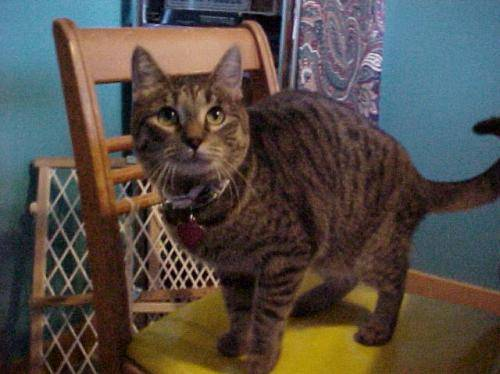
\includegraphics[width=10cm]{../animals_cleaned/cats/cats_00001.jpg}
     \caption{This figure includes a cos function}
         \label{Fig:Fig1}
\end{figure}

%%
Figure \ref {Fig:Fig1} This is the graph containing the cos function.
%%

Tables should be self-explanatory. The table headings should contain 
the essential information needed to understand the data presented. 
Details should not clutter the header and are better added as explanatory 
footnotes. \ref{tab:KapSou} We will see

\begin{table}[htb]
      
     $$ 
         \begin{array}{p{0.7\linewidth}l}
            \hline
            \noalign{\smallskip}
            Source      &  T / {[\mathrm{K}]} \\
            \noalign{\smallskip}
            \hline
            \noalign{\smallskip}
            Yorke 1979, Yorke 1980a & \leq 1700           \\
            Kr\"ugel 1971           & 1700 \leq T \leq 5000 \\
            Cox \& Stewart 1969     & 5000 \leq             \\
            Los Angeles & 3000\\
            Paris & 2\\
            \noalign{\smallskip}
            \hline
         \end{array}
     $$ 
     \caption[]{Example of table caption: opacity sources.}
         \label{tab:KapSou}
\end{table}

\section{Discussion}
In this section you analyse and discuss your results.
This section is paramount as it gives indication about the 
hability of the author to interpret the results and 
critically discuss his or her findings.

\section{Conclusions}
Here you summarize the essential aspects and findings 
of your work and analysis.

Finally, remember to include a section with the bibliography.
It is very important to cite the sources you used for your study and
for writing the report.


% TABLES

\begin{table}[h!]

\begin{center}

\begin{tabular}{l|c|c|r} % <-- Alignments: 1st column left, 2nd middle and 3rd right, with vertical lines in between

\hline
\hline

\textbf{Value 1} & \textbf{Value 2} & \textbf{Value 3}  & \textbf{Value 4}\\

$\alpha$ & $\beta$ & $\gamma$ & $\delta$\\

\hline
\hline

1 & 1110.1 & 100 & a \\

2 & 10.1 & 50 & b \\

3 & 23.113231 & 5 & c \\

800 & 800 & 1 & dd \\

900 & 850 & -10 & ddd \\

\end{tabular}

\caption{Your first table.}

\label{tab:table1}

\end{center}

\end{table}

\begin{table}[ht]

\caption{Partial horizontal line}

\begin{center}

\begin{tabular}{ || c || c || c || c ||}

\hline \hline
% \multicolumn{2}{c}{Multi-column}&\\

% \cline{1-4} 

\rowcolor {red! 50} X&X&X&X\\
\hline \hline
\rowcolor {green! 70} X&X&X&X\\
\hline \hline
\rowcolor {blue! 10} X&X&X&X \\
\hline \hline

\end{tabular}

\end{center}

\label{tab:multicol}

\end{table}

\begin{thebibliography}{}

  \bibitem{baker} Baker, N. 1966,
      in Stellar Evolution,
      ed.\ R. F. Stein \& A. G. W. Cameron
      (Plenum, New York) 333

   \bibitem{balluch} Balluch, M. 1988,
      A\&A, 200, 58

   \bibitem{cox} Cox, J. P. 1980,
      Theory of Stellar Pulsation
      (Princeton University Press, Princeton) 165

   \bibitem{cox69} Cox, A. N.,\& Stewart, J. N. 1969,
      Academia Nauk, Scientific Information 15, 1

   \bibitem{mizuno} Mizuno H. 1980,
      Prog. Theor. Phys., 64, 544
   
   \bibitem{tscharnuter} Tscharnuter W. M. 1987,
      A\&A, 188, 55
  
   \bibitem{terlevich} Terlevich, R. 1992, in ASP Conf. Ser. 31, 
      Relationships between Active Galactic Nuclei and Starburst Galaxies, 
      ed. A. V. Filippenko, 13

   \bibitem{yorke80a} Yorke, H. W. 1980a,
      A\&A, 86, 286

   \bibitem{zheng} Zheng, W., Davidsen, A. F., Tytler, D. \& Kriss, G. A.
      1997, preprint
\end{thebibliography}

\end{document}

